\documentclass{article}
\usepackage[utf8]{inputenc}
\usepackage[spanish]{babel}

% Formato de página
\usepackage[letterpaper, margin = 1.5cm]{geometry}

% Más opciones para enumerar
\usepackage{enumitem}

% Manejo de imágenes
\usepackage{graphicx}
\usepackage{wrapfig}
\graphicspath{{img/}}
\usepackage{float}

\begin{document}
    \title{
        Fundamentos de bases de datos \\
        Tarea 4 \\
        Álgebra Relacional
    }
    \author{
        Díaz Gómez Silvia \\
        Eugenio Aceves Narciso Isaac \\
        Quiroz Castañeda Edgar
    }
    \date {
        3 de abril del 2019    
    }
    \maketitle

    \begin{enumerate}
        \item {
            Para el problema de la base de datos del \textbf{Museo} que se
            transformó a \textbf{Modelos Relacional} en la tarea anterior,
            verifica que con ésta puedas satisfacer las siguientes consultas.
            \begin{figure}[H]
                \centering
                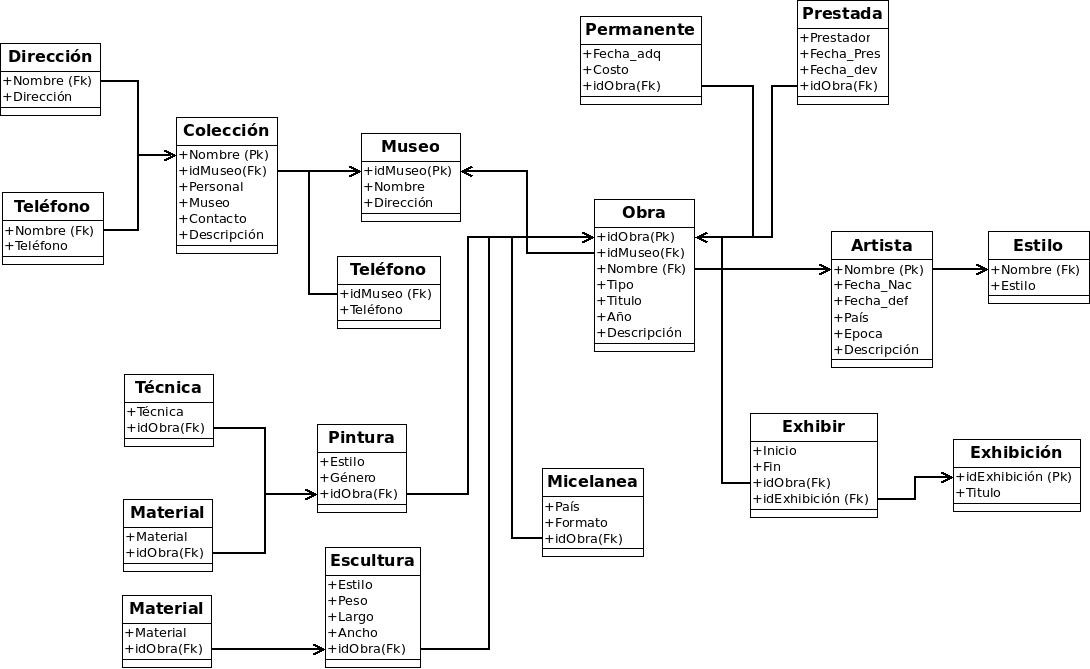
\includegraphics[scale=0.4]{img/museo.jpeg}
                \caption{Esquema relacional del Museo}
            \end{figure}
            \begin{enumerate}
                \item {
                    Toda la información de las obras, nombre del artista que la
                    realizó y país de las obras que se realizaron con estilo
                    Surrealista o Impresionista.
                }
                \item {
                    Una lista con el nombre de los artistas y la cantidad de
                    obras que realizó (entre pinturas, esculturas y miscelánea).
                }
                \item {
                    Lista con la cantidad de obras que se tiene por cada estilo
                    (entre pinturas, esculturas y miscelánea).
                }
                \item {
                    Obtener el año en que menos obras se realizaon y la obra más
                    constosa de ese año.
                }
                \item {
                    Toda información (obras y artistas) de las obras que se
                    obtuvieron en préstamo el 28 de noviembre de año 2014 y que
                    no han sido devuletas.
                }
            \end{enumerate}
            \item {
                Si tienes el siguiente esquema para una Base de Datos:
                \begin{itemize}[label={}]
                    \item \textbf{Empleado}(CURP, nombre, calle, ciudad)
                    \item \textbf{Trabaja}(CURP, idEmpresa, suelo)
                    \item \textbf{Empresa}(idEmpresa, nombre, ciudad)
                    \item \textbf{Jefe}(CURPJ, CURPE)
                \end{itemize}
                Considera que el suelo que reciben los empleados es mensual.
                Escribe una expresión en \textbf{Álgebra Relacional} para cada
                una de las siguientes consultas
                \begin{enumerate}
                    \item {
                        Lista con la \textbf{CURP} y \textbf{nombre} de cada
                        empleado que trabaja en \textbf{Flanders Ship Asociados
                        (FSA)}.
                    }
                    \item {
                        Averiguar el \textbf{nombre} y la \textbf{ciudad de
                        residencia} de todos los empleados que trabajan para el 
                        \textbf{Compumundo Hipermega Red (CHR)}.
                    }
                    \item {
                        El \textbf{nombre}, \textbf{la calle} y la \textbf{ciudad
                        de residencia} de todos los empleados que trabajan para
                        \textbf{FSA} y ganan entre \textbf{\$150,000} y
                        \textbf{\$190,000} anuales.
                    }
                    \item {
                        Encontrar el \textbf{nombre} y \textbf{CURP} de los
                        empleados que vivan en la misma ciudad en que está
                        ubicada la compañia a la que prestan sus servicios.
                    }
                    \item {
                        Lista con el  \textbf{nombre} de los empleados que viven
                        en la \textbf{misma calle} y la \textbf{ciudad} de su
                        \textbf{jefe}.
                    }
                    \item {
                        Averiguar la \textbf{CURP} de los empleados que no
                        trabajan para \textbf{FSA} pero sí para \textbf{CHR}.
                    }
                    \item {
                        Encontrar el \textbf{nombre}, \textbf{CURP} y
                        \textbf{ciudad de residencia} de todos los jefes
                        registrados en la base de datos.
                    }
                    \item {
                        Una lista con el \textbf{nombre} de todos los empleados
                        que trabajan para  \textbf{CHR} pero no para
                        \textbf{FSA}.
                    }
                    \item {
                        Lista con la \textbf{CURP} de los empleados que ganan
                        más que cualquier empleado \textbf{FSA}.
                    }
                    \item {
                        Lista cin el \textbf{nombre de las companías} que están
                        instaladas en una ciudad donde haya un
                        \textbf{Krusty Burger}.
                    }
                    \item {
                        Borrar toda la información de la companía
                        \textbf{Mapple}.
                    }
                    \item {
                        Disminuir el sueldo de los empleados que trabajan en
                        \textbf{Mr. Plow} en un \textbf{8\%}.
                    }
                    \item {
                        Una lista con la \textbf{cantidad de empleados} que se
                        tienen por ciudad y por compañía.
                    }
                    \item {
                        Cambiar la ubicación de \textbf{Sorby} (y de 
                        \textbf{todos sus empleados}) a \textbf{Ciudad Capital}.
                    }
                    \item {
                        A los empleados que trabajan en \textbf{Ziffcorp} y que
                        ganen \textbf{\$18,000 mensuales} hacerles un
                        \textbf{decremento del 8\%}, mientras que a los que
                        trabajan en \textbf{Panaphonics} y que ganen 
                        \textbf{menos de \$12,000 mensuales} aumentarles su
                        sueldo en un \textbf{10\%}.
                    }
                    \item {
                        Lista de los empleados que trabajen en \textbf{más de
                        dos compañías} y el \textbf{número de companías} en que 
                        laboran.
                    }
                    \item {
                        Lista que muestre la \textbf{CURP del jefe} y el
                        \textbf{número de empleados} que están a su cargo,
                        agrupados por companía.
                    }
                    \item {
                        Una lista de los empleados que ganene \textbf{más de 
                        \$140,000 mensuales} y ue \textbf{no viven} en
                        \textbf{Springfield}.
                    }
                    \item {
                        La empresa que paga el mayor \textbf{sueldo promedio}.
                    }
                    \item {
                        \textbf{Moe Szyslak} decide dejar su bar y entrar a
                        trabajar a la planta nuclear, siendo su nuevo jefe
                        \textbf{Carl Carlson}. Refleja estos cambios en la base
                        de datos.
                    }
                \end{enumerate}
            }
        }
    \end{enumerate}
\end{document}